\documentclass[10pt,a4paper]{article}
\usepackage[utf8]{inputenc}

\usepackage[table,xcdraw]{xcolor}
\usepackage[landscape,margin=0.5cm]{geometry}
\usepackage[english]{babel}
\usepackage{subcaption}
\usepackage{tikz-network}
\usepackage{amsmath}
\usepackage{amssymb}
\usepackage{adjustbox}
\usepackage{booktabs}
\DeclareMathOperator*{\argmax}{argmax} % thin space, limits underneath in displays
\DeclareMathOperator*{\argmin}{argmin} % thin space, limits underneath in displays

% colour themes to come. KnitR?

%-------------------------

\title{\huge{Network Science Cheatsheet}}
\author{\small{Remy Cazabet}}
\date{}
\usepackage[default]{raleway}
\usepackage{fontawesome}
\usepackage[T1]{fontenc}

\usepackage{hyperref}
\usepackage{enumitem}
\usepackage{lipsum}

\usepackage{xcolor}
\definecolor{customcolor}{HTML}{616AC5}
\definecolor{alert}{HTML}{CD5C5C}
\definecolor{w3schools}{HTML}{4CAF50}
\definecolor{subbox}{gray}{0.60}
\definecolor{codecolor}{HTML}{FFC300}
\colorlet{xx}{customcolor}


%--------------------------Editor mode.

\usepackage
[%sectionbib,openany,
citestyle=authoryear,
sorting=nty,	  		%Sorts bibliography by year, name, title
autocite=footnote, 		%Autocite command generates footnotes
autolang=hyphen, 		
mincrossrefs=1, 	
backend=biber]
{biblatex}

\DeclareFieldFormat{postnote}{#1}
\DeclareFieldFormat{multipostnote}{#1}
\DeclareAutoCiteCommand{footnote}[f]{\footcite}{\footcites}

\bibliography{literature}
%----------------------------------------
%--------------------------------------------------------------------------------
\usepackage{tcolorbox}

\tcbuselibrary{most,listingsutf8,minted}

\tcbset{tcbox width=auto,left=1mm,top=1mm,bottom=1mm,
right=1mm,boxsep=1mm,middle=1pt}

\newenvironment{mycolorbox}[2]{%
\begin{tcolorbox}[grow to left by=-1em,grow to right by=-1em,capture=minipage,fonttitle=\large\bfseries, enhanced jigsaw,boxsep=1mm,colback=#1!30!white,on line,tcbox width=auto, toptitle=0mm,colframe=#1,opacityback=0.7,nobeforeafter,title=#2]%
}{\end{tcolorbox}\\[0.2em]}

\newenvironment{subbox}[2]{%
\begin{tcolorbox}[capture=minipage,fonttitle=\normalsize\bfseries, enhanced jigsaw,boxsep=1mm,colback=#1!30!white,on line,tcbox width=auto,left=0.3em,top=1mm, toptitle=0mm,colframe=#1,opacityback=0.7,nobeforeafter,title=#2]\footnotesize %
}{\normalsize\end{tcolorbox}\vspace{0.1em}}

\newenvironment{multibox}[1]{%
\begin{tcbraster}[raster columns=#1,raster equal height,nobeforeafter,raster column skip=1em,raster left skip=1em,raster right skip=1em]}{\end{tcbraster}}

\newenvironment{textbox}[1]{\begin{mycolorbox}{customcolor}{#1}}{\end{mycolorbox}}

%-------------------------------
\newtcblisting{codebox}[2]{colback=codecolor!5,colframe=codecolor!80!black,listing only, 
minted options={numbers=left,style=tcblatex,fontsize=\tiny,breaklines,autogobble,linenos,numbersep=3mm},
left=5mm,enhanced,
title=#2, fonttitle=\bfseries,
listing engine=minted,minted language=#1}

%--------------------------------------------------------------------------------
\newcommand{\punkti}{~\lbrack\dots\rbrack~}

\renewenvironment{quote}
               {\list{\faQuoteLeft\phantom{ }}{\rightmargin\leftmargin}%
                \item\relax\scriptsize\ignorespaces}
               {\unskip\unskip\phantom{xx}\faQuoteRight\endlist}
               

%--------------------------------------------------------------------------------
\newcommand{\bgupper}[3]{\colorbox{#1}{\color{#2}\huge\bfseries\MakeUppercase{#3}}}
\newcommand{\bg}[3]{\colorbox{#1}{\bfseries\color{#2}#3}}

\newcommand{\mycommand}[2]{{\ttfamily\detokenize{#1}}~\dotfill{}~{\footnotesize #2}\\}
\newcommand{\sep}{{\scriptsize~\faCircle{ }~}}


\newcommand{\bggreen}[1]{\medskip\bgupper{w3schools}{black}{#1}\\[0.5em]}
\newcommand{\green}[1]{\smallskip\bg{w3schools}{white}{#1}\\}
\newcommand{\red}[1]{\smallskip\bg{alert}{white}{#1}\\}

\usepackage{multicol}
\setlength{\columnsep}{5pt}

\setlength{\parindent}{0pt}
\pagestyle{empty}

\usepackage{csquotes}

\newcommand{\loremipsum}{Lorem ipsum dolor sit amet.}



%--------------------------------------------------------------------------------
\begin{document}

\small
\begin{multicols}{3}

%\maketitle

\thispagestyle{empty}
\scriptsize
%\tableofcontents



\begin{subbox}{subbox}{}
\centering
\Large{\textbf{Network Science   \\ Cheatsheet}}
\end{subbox}

\begin{multibox}{2}
\begin{subbox}{subbox}{}
\centering

\includegraphics[width=0.8\textwidth]{pics/logo.png}
\end{subbox}
\begin{subbox}{subbox}{}
\centering
Made by \\
\large{
Remy Cazabet
}
\end{subbox}
\end{multibox}



% \input{intro}




% \input{matrices}












% \input{centrality}

% \documentclass[addpoints]{exam}
\usepackage[utf8]{inputenc}
\usepackage{xcolor}
\definecolor{light-gray}{gray}{0.95}
\newcommand{\code}[1]{\colorbox{light-gray}{\texttt{#1}}}


\usepackage{tikz,lipsum,lmodern}
\usepackage[most]{tcolorbox}
\usepackage{url}


%This block of commented code translates default words to Spanish
%-------------------------------------------------------------
%\pointpoints{punto}{puntos}
%\bonuspointpoints{punto extra}{puntos extra}

%\totalformat{Pregunta \thequestion: \totalpoints{} puntos}

%\chqword{Pregunta}
%\chpgword{Página}
%\chpword{Puntos}
%\chbpword{Puntos extra}
%\chsword{Puntos obtenidos}
%\chtword{Total}

%\boxedpoints
%-------------------------------------------------------------

\begin{document}
%This code creates the text before the first question
%-------------------------------------------------------------------
\begin{center}
\fbox{\fbox{\parbox{5.5in}{\centering
Experimenting with Scale-Free networks}}}
\end{center}

% \vspace{5mm}
% \begin{tcolorbox}[colback=black!5!white,colframe=white!75!black]
% You can do the exercises in the order that you prefer. \\  
% the \textit{Going further} experiments take more time and I do not expect everyone to do them.
% \end{tcolorbox}
% \vspace{5mm}

%Here, the questions begin
\begin{questions}



\question Generating Scale-Free networks with Preferential Attachment.

\begin{tcolorbox}[colback=black!5!white,colframe=white!75!black]
Networkx has a function to create networks following the preferential attachment principle (\code{barabasi\_albert\_graph}), but we would like to study the dynamic of the model, so we will code our own version.
\end{tcolorbox}
\begin{parts}
\part Using networkx, generate an initial random ER network composed of a small number of nodes
\part Write a \code{for} loop, such as each iteration adds a new node to the network, with a small number of edges, each of them connected to existing nodes with a probability proportional to their degree (\textit{preferential attachment}). You can use, for instance, the method \code{numpy.random.choice}
\part Plot the degree distribution, with and without a \textbf{log-log} scale.
\begin{tcolorbox}[colback=black!5!white,colframe=white!75!black]
Plotting properly power-law distributions can be tricky. A simple way to do it is to use \code{collections.Counter} to count occurences of each degree, and plot the resulting keys and values as a \textit{scatter plot} (x=degree,y=occurences(frequencies))
\end{tcolorbox}
\part We want to observe how node degrees increase over time. For a few nodes (e.g., nodes 1, 2, 3, 9, 10, 11, 19, 20, 21), plot the evolution of their degree, for instance on a plot such as x=iteration, y=degree, one line per node. 
\part Compare the degree distribution after the first, last, and some intermediary steps.
\begin{tcolorbox}[colback=black!5!white,colframe=white!75!black]
To plot several distributions on a same plot, you can either use \code{seaborn.scatterplot}, providing a \textit{long form} pandas dataframe, i.e., a dataframe with 3 columns (x,y,label) such as each row correspond to one point (x,y) of the experiment represented by \textit{label}. The plot is then done calling \code{scatterplot(x="x",y="y",hue="label",data=dataframe)}. Another solution is to call several time pyplot \code{plt.plot(x, y, 'color', label='label')} function.
\end{tcolorbox}
\part Vary the number of initial nodes, the number of nodes to add and the number of edges added by each node, and observe how the final degree distribution is affected.


\end{parts}    



\vspace{5mm}
\question Going further : fitting exponents
%This question has several parts
\begin{parts}
\part We have seen that a power law distribution is defined by its exponent. We would like to find the exponent of our distribution. First, we try to find it manually. The exponent is the slope of the line on a log-log plot. Can you find it \textit{graphically}? (e.g., if you move one unit to the right on the x axis, how many units are you going down on the y axis to stay on the line)
\part Let's try to fit by trial an error. Draw lines corresponding to power law distributions of intersect $C$ and exponent $\alpha$, using the formula of the power law distribution.
\begin{tcolorbox}[colback=black!5!white,colframe=white!75!black]
A simple way to draw distribution is to generate series of values for x, e.g., \code{x = np.arange(1,100, dtype=float)}, and then to compute the y value for each of those x, e.g., \code{y = a*x+b)}
\end{tcolorbox}
\part A naive way to fit the exponent would be to use a least-square regression on log values, i.e., find the slope of the line that we can observe on a log-log plot. You can use for instance the \code{LinearRegression} method of package sklearn, \code{model = LinearRegression.fit(log\_x,log\_y)}, with log\_x and log\_y being the log values of observed x and y. Intercept and exponent can be obtained with \code{model.intercept\_} and \code{model.coef\_}. 
\part Plot the line and check how well it fits the model. If you're not satisfied, try to impose min and max values of degree to consider.
\part Fitting power laws with least square is known to be tricky. The \code{powerlaw} package has been developed to help doing it properly. Using the documentation \url{https://pythonhosted.org/powerlaw/}, use the package to find the exponent of your distribution. How close is it from your previous experiments? Which one corresponds the most to what is known in theory about the exponent of the prefential attachment model?
\end{parts}




\end{questions}


\end{document}

%











\begin{textbox}{Assortativity - Homophily}

A network is said to be \textbf{assortative} or to demonstrate \textbf{homophily} if its nodes tend to connect more with other nodes that are \textbf{similar} than to nodes that are different. 

Similarity in this case must be understood in term of nodes properties. Some typical examples can be age, gender, language, political beliefs, etc.

Homophily is considered a common feature of many networks, in particular social networks, as reflected in the aphorism \textit{Birds of a feather flock together}.

Some networks can also demonstrate \textbf{heterophily}, or \textbf{disassortativity}, i.e., a greater number of connections with nodes that are different (for instance, in a sentimental relationship network, women tend to connect more with men than with other women).



\end{textbox}


\begin{textbox}{Note on interpreting homophily}
Homophily can be a link creation mechanism (nodes have a preference to connect with similar ones, so the network end up to be assortative), or a consequence of influence phenomenons (because nodes are connected, they tend to influence each other and thus become more similar).

Without access to the dynamic of the network and its properties, it is not possible to differentiate those effects.


\end{textbox}

\begin{textbox}{Homophily for categorical variables}
When the property for which we study homophily is \textbf{categorical}, i.e., there is no natural order between values, homophily is defined by counting the number of edges that connect two nodes of the same category. The assortativity score is computed by dividing the observed number of such edges to the expected number of such edges in a random network of similar properties, i.e., respecting distributions of each category. More formally, it is expressed as:

\[
r=\frac{\sum_i e_{ii} - \sum_i a_i b_i}{1- \sum_i a_i b_i}
\]
where $e_ii$ is the fraction of edges connecting two nodes of category $i$, $a_i=b_i$ the fraction of nodes of category $i$. Note that $a_i$ and $b_i$ can also be different in a bipartite network, for instance.

Let's see a fictional example. Columns/Rows correspond to blood types, and numbers are expressed in fraction of the total population, while edges represent a social interaction.

\centering
\begin{tabular}{|
>{\columncolor[HTML]{EFEFEF}}l |
>{\columncolor[HTML]{FFFFFF}}l 
>{\columncolor[HTML]{FFFFFF}}l 
>{\columncolor[HTML]{FFFFFF}}l 
>{\columncolor[HTML]{FFFFFF}}l 
>{\columncolor[HTML]{EFEFEF}}l |}
\hline
Blood Types & \multicolumn{1}{l|}{\cellcolor[HTML]{EFEFEF}A} & \multicolumn{1}{l|}{\cellcolor[HTML]{EFEFEF}AB} & \multicolumn{1}{l|}{\cellcolor[HTML]{EFEFEF}B} & \multicolumn{1}{l|}{\cellcolor[HTML]{EFEFEF}O} & $a_i$        \\ \hline
A           & \cellcolor[HTML]{ECF4FF}0.30                   & 0.05                                            & 0.1                                            & 0.05                                           & \textit{0.5} \\ \cline{1-1}
AB          & 0.05                                           & \cellcolor[HTML]{ECF4FF}0.05                    & 0                                              & 0                                              & \textit{0.1} \\ \cline{1-1}
B           & 0.1                                            & 0                                               & \cellcolor[HTML]{ECF4FF}0.2                    & 0                                              & \textit{0.3} \\ \cline{1-1}
O           & 0.05                                           & 0                                               & 0                                              & \cellcolor[HTML]{ECF4FF}0.05                   & \textit{0.1} \\ \cline{1-1}
$b_i$      & \cellcolor[HTML]{EFEFEF}\textit{0.5}           & \cellcolor[HTML]{EFEFEF}\textit{0.1}            & \cellcolor[HTML]{EFEFEF}\textit{0.3}           & \cellcolor[HTML]{EFEFEF}\textit{0.1}           & \textbf{1}   \\ \hline
\end{tabular}

\vspace{0.3cm}

$r=\frac{(0.3+0.05+0.2+0.05)-(0.5^2+0.1^2+0.3^2+0.1^2)}{1-(0.5^2+0.1^2+0.3^2+0.1^2)}=\frac{0.6+0.36}{1-0.36}=0.375$

\vspace{0.3cm}

$r=0$ means that the network has no assortative mixing, $r=1$ corresponds to a perfectly assortative network (edges exist only between nodes of the same category), and $r=1$ to a perfectly disassortative network (no edge between nodes of the same category).
\end{textbox}











\begin{textbox}{Homophily for numerical variables}
When the property for which we study homophily is \textbf{numerical}, homophily $r$ is defined as the person correlation coefficient between values at both end of each nodes. For details, see \cite{newman2003mixing}.

\vspace{0.3cm}


Homophily $r=0$ means that the network has no assortative mixing, $r>0$ corresponds to an assortative network (nodes with high values tend to connect to high values), and $r<0$ to a disassortative network (nodes with high values are preferably connected to low values).

\end{textbox}













\begin{textbox}{Degree assortativity}
\textbf{Degree assortativity}, sometimes simply called \textit{assortativity}, is a particular case of homophility measuring homophily in term of node degrees, i.e., the numerical value of each node is its degree.

The existence of a degree assortativity can be interpreted in term of a \textit{rich club phenomenon}: hubs prefer to connect to other hubs.

\end{textbox}



% \begin{textbox}{Neighbor connectivity }
% \textbf{Neighbor connectivity} is another way to study the correlation between node degrees. The principle is to study how the degree of nodes relates to the average degree of its neighbors, i.e., the relation between $k_u$ and \frac{1}{|N_u|}$\sum_{v\in N_u} k_v$ for all $u$. The sign of the correlation between those variables inform about the 

%%%% Be careful, check the relation with the friendship paradox
% \end{textbox}








% \documentclass[a4paper,11pt]{book}
\usepackage{import}
\usepackage{preamb}

\makeindex

\begin{document}

\small
\begin{multicols}{3}

%\maketitle

\thispagestyle{empty}
\scriptsize
\newpage


\begin{subbox}{subbox}{}
\centering
\Large{\textbf{Network Science   \\ Cheatsheet}}
\end{subbox}

\begin{multibox}{2}
\begin{subbox}{subbox}{}
\centering

\includegraphics[width=0.8\textwidth]{pics/logo.png}
\end{subbox}
\begin{subbox}{subbox}{}
\centering
Made by \\
\large{
Remy Cazabet
}
\end{subbox}
\end{multibox}
% \section{Blocks and Community structure}


\begin{subbox}{subbox}{}
\centering
\Large{\textbf{Random Graphs}}
\end{subbox}


\begin{subbox}{subbox}{}
\centering
Many elements of this course are inspired by the excellent classes by Aaron Clauset, than can be found online:  \url{ http://tuvalu.santafe.edu/~aaronc/courses/5352/}  \end{subbox}








\begin{textbox}{Synthetic networks usages}

Using synthetic networks is essential in network science for several reasons. In particular, they allow to:
\begin{itemize}
    \item Study some properties in a \textbf{controlled environment}. \textit{What happens if we increase property $X$, while keeping all other properties constant?}
    \item Compare an observed network with a \textbf{randomized} version of it. \textit{I observed property X in my data, is it something remarkable, or would I observe the same thing on a random network similar to my graph?}
    \item Explain a phenomenon. \textit{Property X seems exceptional. It can be reproduced in random networks by simple mechanism Y.}
    \item Generate synthetic datasets, for instance to test the same algorithm on multiples variations of the same network.
\end{itemize}

\end{textbox}




\begin{textbox}{Synthetic networks types}
There are three main types of synthetic networks:
\begin{itemize}
    \item \textbf{Deterministic models} are instances of famous graphs or, more commonly, repeated regular patters. e.g., \textit{Caveman graph, grids, lattices}.
    \item \textbf{Generative models} assign to each pair of nodes a probability of having an edge according to their properties (degree, label, etc.). e.g., \textit{Erdős Rényi, Configuration model, etc.} 
    \item \textbf{Mechanistic models} create networks by following a set of rules, a process defined by an algorithm. e.g., \textit{Preferential attachment, Forest fire, etc.}
\end{itemize}
\end{textbox}






\begin{textbox}{Regular lattices}
Regular lattices are defined as repetition of the same pattern a given (potentially infinite) number of times. Nodes all have the same degree. The pattern can be in 1, 2 or more dimensions. 

The \textbf{clustering coefficient} depends on the structure, it can be large if the structure is made of triangles, for instance. It is the same for all nodes (except potentially nodes at the boundaries).

The \textbf{average distance} grows quickly with $n$, if $k \ll n$
\end{textbox}


\begin{textbox}{Erdős-Rényi (ER) model}
The \textbf{Erdős-Rényi (ER)} model is the simplest random graph model. Assuming that we know the number of nodes and the number of edges, and no other information, then edges are simply put between randomly chosen pairs of nodes.

ER models can be defined in two ways:
\begin{itemize}
    \item in the $G(n,L)$ formulation, the number of edges of the generated graph is set to exactly $L$, and thus $L$ random pairs of nodes are chosen among the set of all existing node pairs (sharp constraint, microcanonical ensemble).
    \item in the $G(n,p)$ formulation, an edge is added between any set of node with a probability $p$. (soft constraint, canonical ensemble).
\end{itemize}

Properties of both model are similar when the number of edges (defined by $L$ or $p$) is large.

\end{textbox}








\begin{textbox}{Random version of observed graph}
When one wants to compare a real network with a \textbf{randomized} version of it (also called a \textbf{rewired} network), the usual way is not to start from the original network and to actually rewire it edge by edge, but instead to generate a new ER random graph keeping the same number of nodes and the same number of edges (or the same density) as the observed network. Properties of the observed network can then be compared with the generated network. Note that it does note make sense to compare the properties of any particular node in both networks, since nodes in the random graph have no identity. For many applications, there is not need to actually generate a random graph: one can simply compare properties of the real network with theoretical properties of the random graph.

\end{textbox}









\begin{textbox}{Soft ER}
In the soft ER, the number of edges is not known in advance. The distribution of the number of edges in the soft ER is described by the \textbf{binomial distribution} $\mathbb{B}(L^{max},p)$



From the known properties of the Binomial distribution, it can be shown that:
\begin{itemize}
    \item The \textbf{expected number of edges} is $\langle L \rangle = p L^{max}$, 

    \item The \textbf{variance of the number of edges} is $\sigma^2 = L^{max}p(1-p)$
\end{itemize}

\end{textbox}



\begin{subbox}{subbox}{Binomial distribution}
 The \textbf{Binomial distribution} $\mathbb{B}(N_b,p_b)$ is a discrete distribution modeling the number of successes $x$ in a sequence of $N_b$ independent experiments with success probability $p_b$. For instance, it models how many times ($x$) one will obtain a 6 (\textit{success}) if they throw a dice $N_b$ times and that the probability to obtain a 6 is $\frac{1}{6}$. It is defined as $P(x)=\binom{N_b}{x}p^x(1-p_b)^{N-x}$. $\binom{N}{x}$ is the binomial coefficient, describing the number of ways, disregarding order, that $x$ elements can be chosen among $N_b$.
\end{subbox}





\begin{textbox}{ER: Degree distribution}
Since each node has an independent probability to be connected with each other node, the degree distribution of the ER model is modeled as a binomial distribution $\mathbb{B} (N-1 , p)$, i.e., the probability to have a given degree knowing that we have a probability $p$ to have a link with each of the other nodes in the graph. From the properties of the Binomial distribution, we know that:
\begin{itemize}
    \item The \textbf{expected average degree} is $\langle k \rangle=p(N-1)$
    \item The \textbf{variance of the degree} is $\sigma^2_k =p(N-1)(1-p)$
\end{itemize}

\begin{subbox}{subbox}{}
We can note that the distribution becomes increasingly narrow as the network size increases, i.e., we are increasingly confident that the degree of a node is in the vicinity of $\langle k \rangle$: 
\[
\frac{\sigma_k}{\langle k \rangle}=\frac{1}{(N-1)^{1/2}}
\]
\end{subbox}

\end{textbox}


\begin{textbox}{ER: Approximation of degree distribution by a Poisson Distribution}
When the number of nodes $N$ is large and the average degree $\langle k \rangle$ is small, the degree distribution can be approximated by a Poisson distribution $\operatorname {Pois}(\langle k \rangle)$. From the properties of Poisson distributions, we approximate that for a network with average degree $\langle k \rangle$:
\begin{itemize}
   % \item The \textbf{Degree distribution} is $P(k)=\frac{\langle k \rangle^ke^{-\langle k \rangle}}{k!}$
    \item The \textbf{variance of the degree} is $\sigma_k^2 \approx{\langle k \rangle}$
\end{itemize}

\end{textbox}


\begin{subbox}{subbox}{Poisson distribution}
  The \textbf{Poisson distribution} $\operatorname {Pois}(\delta)$ is a discrete distribution modeling the probability of observing exactly $x$ occurrences of an event in a period of duration $\Delta_t$ if this event occurs randomly and that there are in average $\delta$ occurrences of it during a period $\Delta_t$. Working with the Poisson distribution is convenient because it depends only on a single parameter $\delta$. %It is known that the Poisson distribution is a good approximation of the Binomial when $N_b$ is large and $p_b$ is small, which is the case for sparse graphs.
\end{subbox}













\begin{textbox}{ER: Clustering Coefficient}
The \textbf{Global Clustering Coefficient} of a network is defined as the fraction of closed triads among all triads. Since any edge $(u,v)$ has a fix probability to exist $p$ independently of the existence of any other edge in the network, the probability of having edge $(a,c) \in E$ for a triad $[a,b,c]$ such as $(a,b),(b,c) \in E$ tends towards $p$ for large graphs. 

Thus, the clustering coefficient of an ER graph is $C^g\approx p$. Since we know that most real networks are sparse, $p$ is small, thus $C^g$ is small. A similar reasoning can be used to show that the average clustering coefficient $\langle C \rangle$ is small too.  

\end{textbox}


\begin{textbox}{ER: Average Distance}
We can intuitively estimate the order of the \textbf{Average Distance} of an ER random graph as follows: 

We know that the clustering coeffient of an ER graph is small. Therefore, we can approximate the graph as having a tree-like structure. As a consequence, the number of nodes located at distance $d$ of a node $u$ increases as $\langle k \rangle^d$. From this approximation, the relation between distance and number of nodes is $N=\langle k \rangle^d$ hops, thus the order of $\ell$ is  $\log_{\langle k \rangle}n=\frac{\log N}{\log \langle k \rangle}$.

We can thus say that the order of the average distance of a sparse ER graph relatively to its size is $\mathcal{O}(log N)$, and thus that: \textbf{ER graphs have a short average distance}.



\end{textbox}


\begin{subbox}{subbox}{Order of magnitude}
 The notation $\mathcal{O}$ is used to represent the \textbf{order of magnitude} of a value. It roughly indicates how this value is related to another one, ignoring any constant. For instance, $\mathcal{O}(x)=\mathcal{O}(10x)=\mathcal{O}(x/10)$. Typical orders of magnitude are $\mathcal{O}(\log x)$, $\mathcal{O}( x)$, $\mathcal{O}(x^2)$ and $\mathcal{O}(2^x)$.
\end{subbox}







\begin{textbox}{ER: Largest connected component}

The largest connected component of a graph is a way to measure its connectivity. On random networks, the relation between the density (or average degree) of a graph and the size of its largest connected component is known to undergo a \textit{phase transition} phenomenon, i.e., a rapid change when a threshold is crossed. More precisely, as long as $\langle k \rangle<1$, several connected components of similar sizes exist in the network, while, when  $\langle k \rangle>1$, the graph has a single \textit{giant component} with high probability.

\begin{center}
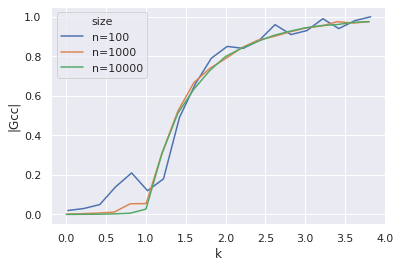
\includegraphics[width=0.8\textwidth]{pics/largestCC.png}
\end{center}

An intuitive way to understand this phenomenon is to use the same observation of the graph being tree-like as previously. Since the number of nodes $N$ that can be reached after $d$ hops can be estimated to grow as $\langle k \rangle^d$, a value of $\langle k \rangle<1$ leads to an impossibility to reach all nodes even for a large $d$, while $\langle k \rangle>1$ leads to arbitrarily large $N$ for long enough $d$. Proper demonstration and more details can be found in the original paper  \footcite{erdHos1960evolution}.

\noindent\rule{4cm}{0.1pt}

You can explore this property using this interactive \textit{explorable}: \url{https://www.complexity-explorables.org/explorables/the-blob/}
\end{textbox}








\begin{textbox}{Configuration Model (CM)}
The \textbf{Configuration Model} is another classic random graph model in which the degree of each node --or the degree distribution-- is preserved. In general terms, a configuration model is defined by the number of nodes in the graph, the number (or probability) of edges, and a distribution of degrees of nodes. 

This degree distribution can either be chosen \textit{a priori}, for instance following a \textit{Poisson} or a \textit{Power-law} distribution, or by taking the observed distribution of a real network we would like to obtain a randomized-version of.

Note that in the later case, nodes can be considered to retain their identity: one can compare the local properties of the node of highest degree between the two graphs, for instance.
\end{textbox}




\begin{textbox}{Why the configuration model}
For many real graphs, nodes represent real entities, and the degree of those nodes is due to an intrinsic property of those nodes, which is known in advance and should be taken into account. For instance, let's consider a network representing flight connections between airports: each node represents an airport, and there is an edge between two airports if a direct flight exist between them. \textit{JFK} international airport in New-York will likely be a Hub in this network, having a very large degree. This large degree is a consequence of the properties of the city it belongs to: large population, touristic attraction, etc. So, \textit{if connections between airports were random}, it could nevertheless be relevant to keep the degree of this node.

Furthermore, the degree distribution itself is also a characteristic of the network: the fact that hubs \textit{do exist} in the network change its properties, compared with a network in which such nodes do not exist.
\end{textbox}











\begin{textbox}{Approximate/Soft Configuration model}
In the approximate version of the Configuration model, each pair of node is connected by an edge with a given probability, which depends on their \textbf{objective degrees}. 

More precisely, the probability of having an edge $(i,j)$ is defined as $p_{uv}= \frac{k_u k_v}{2L}$. Note that this is a well defined probability only if $\max(k_u)^2 < 2m$, otherwise it can be higher than 1. $p_{uv}$ should therefore rather be understood as the \textit{expected number of edges} in a multigraph.

Intuitively, this definition can be understood as follows: each node $u$ has $k_u$ stubs. The total number of stubs in the graph is $2L$. Knowing that node $v$ has $k_v$ stubs, the probability for each stub of $u$ to connect to a stub of $v$ is $\frac{k_v}{2L}$.

Note that this model is defined such as self-loops can exist.

\end{textbox}









\begin{textbox}{Rewired exact configuration model}
When the objective of a configuration model is to obtain a randomized version of an observed graph, a common approach is to fix the exact degree of each node, and to connect \textit{stubs} randomly. An efficient way to do so is to use the following algorithm:

1) Create a list $s$ such as it contains $k_u$ times the index of node $u$ -  2) Randomize $s$ -      3)For each $i$ in $[0,L]$, create an edge between nodes of index $s_{2i}$ and $s_{2i+1}$.

\begin{center}
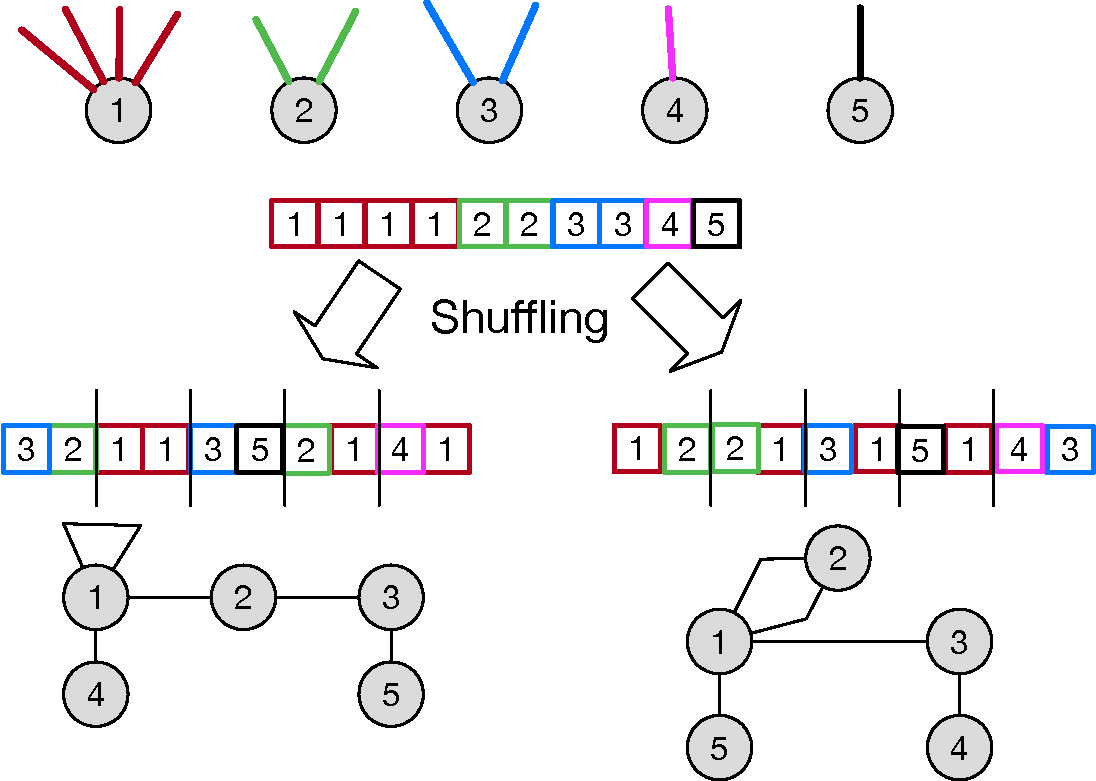
\includegraphics[width=0.5\textwidth]{pics/dynamic/configuration.pdf}
\end{center}

Note that this method can create self-loops and multiple links between the same nodes, even if the original network was a \textit{simple graph}. However, the number of multiple links and self-links decreases when the number of nodes increases, for sparse graphs.

The probability of an edge to exist between two nodes depends on their degree, and is the same as in the soft CM.

For more details on configuration models with fixed degree sequences, see \footcite{fosdick2018configuring}.
\end{textbox}




\begin{textbox}{CM: Clustering Coefficient}
The clustering coefficient of the configuration model can also be studied theoretically. Its derivation is beyond the scope of this class and can be found in the literature \footcite{newman2018networks}. Intuitively, we can use the same reasoning as for the ER model: the probability of having edge $(a,c) \in E$ for a triad $[a,b,c]$ such as $(a,b),(b,c) \in E$ is $\frac{k_a k_c}{2L}$. However, the probability of observing $(a,b)$ and $(b,c)$ and thus to have such a triad also depends on $k_a,k_b,k_c$. In the end, the clustering coefficient is
\[
C = \frac{1}{L}\frac{[\langle k^2 \rangle-\langle k \rangle]^2}{\langle k \rangle^3}
\]

where $\langle k^2 \rangle$ correspond to the expected \textit{variance} (second moment) of the degree.

Since the right part of the equation is a constant depending only on the average degree, the order of the clustering coefficient is $\mathcal{O}(1/L)$, and thus small for large graphs. This is true as long as $\langle k^2 \rangle$ is definite, which might not be the case if the degree distribution is a \textit{power law}.
\end{textbox}





\begin{textbox}{CM: Friendship paradox}
An interesting property of the Configuration Model with heterogeneous degree distribution arises when we study the \textbf{average degree of random neighbors}. Let's call $p_k$ the probability to pick a node of degree $k$ when we pick a node at random. This probability represents the \textit{degree distribution} chosen for the configuration model. Now, if we choose one node at random, and then pick one of its neighbors at random, what is $p_{neighb,k}$, the degree distribution of \textit{random neighbors}? It is different, because nodes with a higher degree have, by definition, a higher probability of being chosen. More formally, 
\[
p_{neighb,k}=\frac{k}{2m}n p_k=\frac{k p_k}{\langle k \rangle}
\]
because $np_k$ is the number of nodes of degree $k$ in the graph, and $\frac{k}{2m}$ is the probability to pick at random a \textit{stub} of a particular node of degree $k$ among all stubs. 

\vspace{0.25cm}

We can now compute the \textbf{average degree of neighbors} of a node chosen at random, as: 
\[
\langle k_{neighb} \rangle = \sum_k k p_{neighb,k} = \frac{\langle k^2 \rangle}{\langle k \rangle}
\]

Thus if all degrees are the same (\textit{homogeneous}), $\langle k_{neighb} \rangle=\langle k \rangle$, but if it is \textbf{heterogeneous}, $\langle k_{neighb} \rangle>\langle k \rangle$ due to the comparatively larger influence of high degrees.


\begin{center}
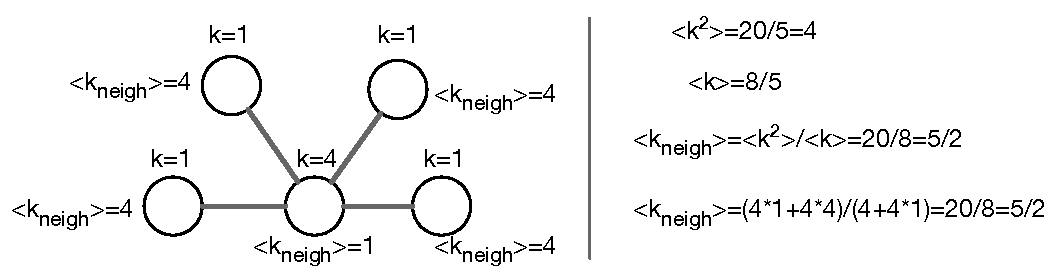
\includegraphics[width=0.9\textwidth]{pics/friendship.pdf}
\end{center}
\end{textbox}







\begin{textbox}{CM: Average distance}
We use the same logic as for the ER model of the graph being locally tree-like due to the low Clustering Coefficient to show intuitively that the \textit{average distance} is short. This property is verified experimentally.
\end{textbox}


\begin{textbox}

Examples of differences in Clustering and average path length for a few real graphs, compared with randomized versions of it.

\tiny
\tabcolsep=0.05cm

\begin{tabular}{lrrrrrrrrr}
\toprule
        graph &   $N$ &   $L$ &   $k$ &  $C_g$ &  $\langle \ell  \rangle$ &  ER-$C_g$ &  ER-$\langle \ell  \rangle$ &  CM-$C_g$ &  CM-$\langle \ell  \rangle$ \\
\midrule
       karate &    34 &    77 &  4.53 &   \textbf{0.26} &                     2.42 &      \textit{0.14} &                        2.42 &      \textit{0.14} &                        2.55 \\
     football &   115 &   613 & 10.66 &   \textbf{0.41} &                     2.51 &      \textit{0.10} &                        2.25 &      \textit{0.07} &                        2.28 \\
 wiki-science &   687 &  6523 & 18.99 &  \textbf{ 0.47} &                     3.43 &      \textit{0.03} &                        2.55 &      \textit{0.08} &                        2.65 \\
     euroroad &  1174 &  1417 &  2.41 &   0.03 &                    \textbf{18.40} &      0.00 &                        7.66 &      0.00 &                        9.55 \\
\bottomrule
\end{tabular}

\end{textbox}




\begin{textbox}{Differences btw. Real \& Random networks}
When comparing real networks to ER and CM networks of similar properties, we observe that they tend to disagree on one of two key properties: on real graphs, usually, the graph has a high clustering coefficient and a short average distance (or sometimes the opposite). 

On the contrary, random networks have both a low clustering coefficient and a short average distance.  

\end{textbox}




\begin{textbox}{Watts-Strogatz (WS) Model}
The Watts-Strogatz model was introduced \footcite{watts1998collective} to show how a simple phenomenon could create networks having both a large clustering coefficient and a short average distance.

The model has 3 parameters:
\begin{itemize}
    \item $N$: number of nodes
    \item $K$: initial number of neighbors
    \item $p$: rewiring probability
\end{itemize}

The network is created following a 2-step processes: first $N$ nodes are disposed on a ring, and each node is connected to its $K$ closest neighbors. Then each edge is replaced by a random edge with probability $p$. It can be interpreted as a network combining the properties of a (1-dimentional) \textbf{regular lattice} and of an \textbf{ER network}.


\end{textbox}


\begin{textbox}{WS - Illustration}
From left to right: WS graphs when increasing the probability of rewiring. $N=20$,$K=4$
\centering
\begin{figure}[H]

\begin{subfigure}{.32\textwidth}
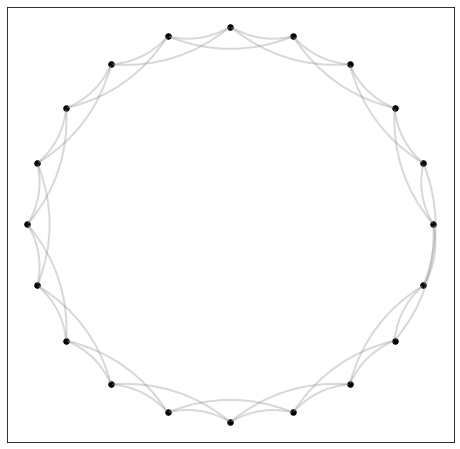
\includegraphics[width=\textwidth]{pics/SW/WS0.png}
    \caption{$p=0$ \\ Regular}
\end{subfigure}
\begin{subfigure}{.32\textwidth}
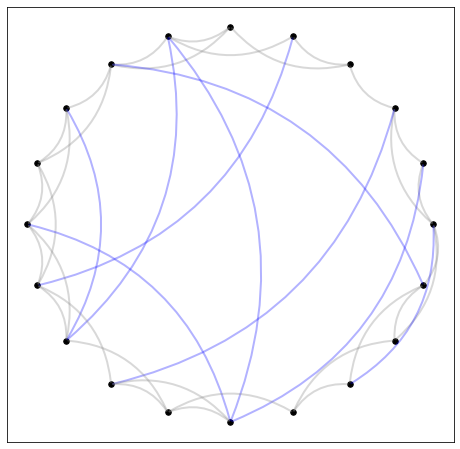
\includegraphics[width=\textwidth]{pics/SW/WS1.png}
    \caption{$p=0.3$ \\ Small world}
\end{subfigure}
\begin{subfigure}{.32\textwidth}
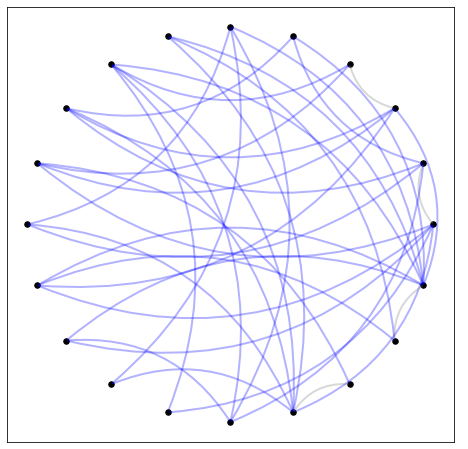
\includegraphics[width=\textwidth]{pics/SW/WS03.png}
    \caption{$p=1$ \\ Random}
\end{subfigure}

\end{figure}

\end{textbox}






\begin{textbox}{WS - Small World Regime}
If $p$ is small, the network has properties similar to a regular lattice, and if $p$ is large, properties of an ER graph.

We can observe this transition by comparing how the Clustering (C) and average distance (d) change when varying $p$, compared with the network when $p=0$, i.e., a regular lattice. 
\begin{center}
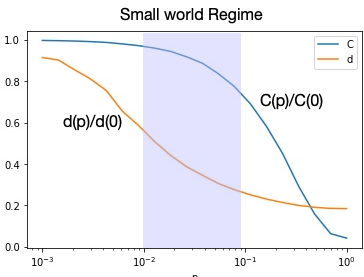
\includegraphics[width=0.6\textwidth]{pics/SW/SWregimes.png}
\end{center}
Example with $N=200, K=6$.
\end{textbox}







\begin{textbox}{WS - Clustering}
Properties of the WS model are not as simple to study theoretically as previous random graphs, so most details are not presented here.
It can be shown however, that the global clustering coefficient can be approximated by:
\[
C^g=\frac{3(K-2)}{4(K-1)+8Kp+4Kp^2}
\]
which is independent of N, thus can be large even for large graphs.
\end{textbox}


\begin{textbox}{WS - Average Path length}
The average path length of the WS model has been studied through approximations and numerical simulations \footcite{newman2000models} and can be shown to become small quickly with the increase in $p$.
\end{textbox}





\begin{textbox}{WS - Degree distribution}
Without entering into details, it can be shown the the degree distribution range from a fixed degree for all nodes to a Poisson distribution, since each rewired edge is decreasing the degree of some nodes and increasing the degree of some others in a random way.
\end{textbox}





\begin{textbox}{Barabási-Albert (BA) Model}
The \textbf{Barabási-Albert} model of random graphs was introduced\footcite{barabasi1999emergence} to illustrate how a simple mechanism could explain a common property of real graphs, the \textbf{power-law degree distribution}.
This mechanism is though to somewhat mimic what is happening in real life, at least for some networks. It is often called \textbf{preferential attachment}, and mimic the \textbf{rich get richer phenomena}: nodes that already have a large degree are more \textit{attractive}, and thus are more likely to become connected with other nodes creating links.
\end{textbox}




\begin{textbox}{BA - Preferential attachment }
The preferential attachment process has two parameters, the number of edges to create at each step $m$ and the initial number of nodes $m_0$, with $m\leq m_0$. It is defined by the following iterative process:
\begin{itemize}
    \item Start with a connected graph with $m_0$ nodes
    \item At each step, add a new node and $m$ links connecting it to $m$ other nodes chosen randomly proportionnaly to their degree, i.e., with probability $p_i=\frac{k_i}{\sum_j k_j}$
\end{itemize}
\end{textbox}

\begin{textbox}{BA - Degree distribution }
The degree distribution created by the preferential attachment mechanism is a power law of exponent $ \alpha=3$. The exponent of the distribution does not depend on parameters $m$ and $m_0$. The degree exponent is \textit{stationary in time}, i.e., it stays the same while we add new nodes and edges.

\noindent\rule{4cm}{0.1pt}

Nodes degree increase with time: the earlier a node was added, the larger its degree tends to be. %More generally, degrees increase as power-law of exponent $\alpha=1/2$

\end{textbox}





\begin{textbox}{BA - Average Path Length }
Networks generated by the BA process have a power-law degree distribution of exponent $ \alpha=3$. It is known that such networks have a short average path length, more formally:
\[
\langle \ell \rangle=\frac{\ln N}{\ln \ln N}
\]

\end{textbox}


\begin{textbox}{BA - Clustering Coefficient }
Although the demonstration is beyond the scope of this class \footcite{barabasi1999emergence}, it can be shown that the clustering coefficient of BA graphs is:
\[
C=\frac{L}{4}\frac{(\ln N)^2}{N}
\]

This is more than for a random network, but still decreases with the network size, and tends toward 0 for large graphs. It is thus considered a \textbf{small} clustering coefficient.

\end{textbox}




\begin{textbox}{Other random graph models }
Many other graph models have been proposed in the literature, either \textit{mechanistic models} to mimic common properties of some graphs, as with BA and WS models, or \textit{statistical models} to generate random graphs with imposed constraints, as the Configuration model does with degree distributions. 

Some examples of mechanistic models:
\begin{itemize}
    \item Vertex copying model (\cite{kleinberg1999web})
    \item Tunable-clustering scale-free model (\cite{holme2002growing})
    \item Forest fire model (\cite{leskovec2005graphs})
\end{itemize}


Some examples of statistical models:
\begin{itemize}
    \item Exponential Random Graphs (\cite{robins2007introduction})
    \item Stochastic Block Models (\cite{peixoto2019bayesian})
    \item A survey on the topic (\cite{orbanz2014bayesian})
\end{itemize}
\end{textbox}








% \begin{textbox}{Vertex-copying model}
% Although the demonstration is beyond the scope of this class \footcite{barabasi1999emergence}, it can be shown that the clustering coefficient of BA graphs is:
% \[
% C=\frac{L}{4}\frac{(\ln N)^2}{N}
% \]

% This is 5 times more than for a random network, but still decreases with the network size, and vecomes very small for large graphs. It is thus considered a \textbf{small} clustering coefficient.

% \end{textbox}



 \AtNextBibliography{\footnotesize}


\printbibliography[heading=subbibliography]


\end{multicols}



\end{document}






% \input{communities}



















































































% \begin{textbox}{Edge Centralities}

% O_{ij} & \textbf{Link Clustering coefficient}


% \end{textbox}


























% \begin{textbox}{Networks: Matrix notation}

% Adjacency matrix $A$
% \begin{itemize}
%     \item $A_{ij}=0$ if link (i,j) does not exist. Otherwise, 1 (unweighted networks), or a number (weight)
%     \item $A$ is symmetric if the network is undirected
% \noindent\rule{4cm}{0.1pt}

% \tiny{More on matrices in \ref{matrix}}

% \end{itemize}
% \end{textbox}
















% \begin{textbox}{Random Graphs models}

% \textbf{Erdos Renyi}

% \textbf{Watts-Strogatz}

% \textbf{Configuration Model}

% \textbf{Stochastic Block Model}

% \end{textbox}











































% \begin{textbox}{Community Detection}

% \textbf{Modularity}
% Divisive

% Agglomerative
% Louvain

% Overlapping
% CPM

% \textbf{Random Walk Compression - Infomap}

% \textbf{SBM inference}


% \end{textbox}


% \begin{textbox}{Key concepts I}
% \red{Bag-of-words (BOW)}

% \green{\emph{type} vs. \emph{token}}
% \emph{To be or not to be.} = 6 \emph{tokens}, 4 \emph{types}.

% \red{\emph{type}} descriptive criterion\footcite[cf.][12]{stroustrup}

% \red{\emph{token}} unit of analysis\footcites[cf.][12]{stroustrup,attentionMerchants}


% \bigskip

% \underline{Key topics}
% \begin{itemize}
%     \item One
%     \item Two
%     \item Three
% \end{itemize}

% \end{textbox}









% %--------------------------------------------------------------
% \section{Tools}



% \begin{textbox}{Lorem Ipsum}
% test  \sep test \sep test \sep test

% \bigskip

% \green{Visualize}
% \begin{enumerate}
% \item \textbf{present} your data
% \item \textbf{analyze} the information
% \item \textbf{explore} the findings
% \end{enumerate}

% \end{textbox}


% \begin{textbox}{Voyant Tools}
%  \href{https://voyant-tools.org/}{Voyant Tools} \sep \href{https://voyant-tools.org/}{Voyant Tools}

% 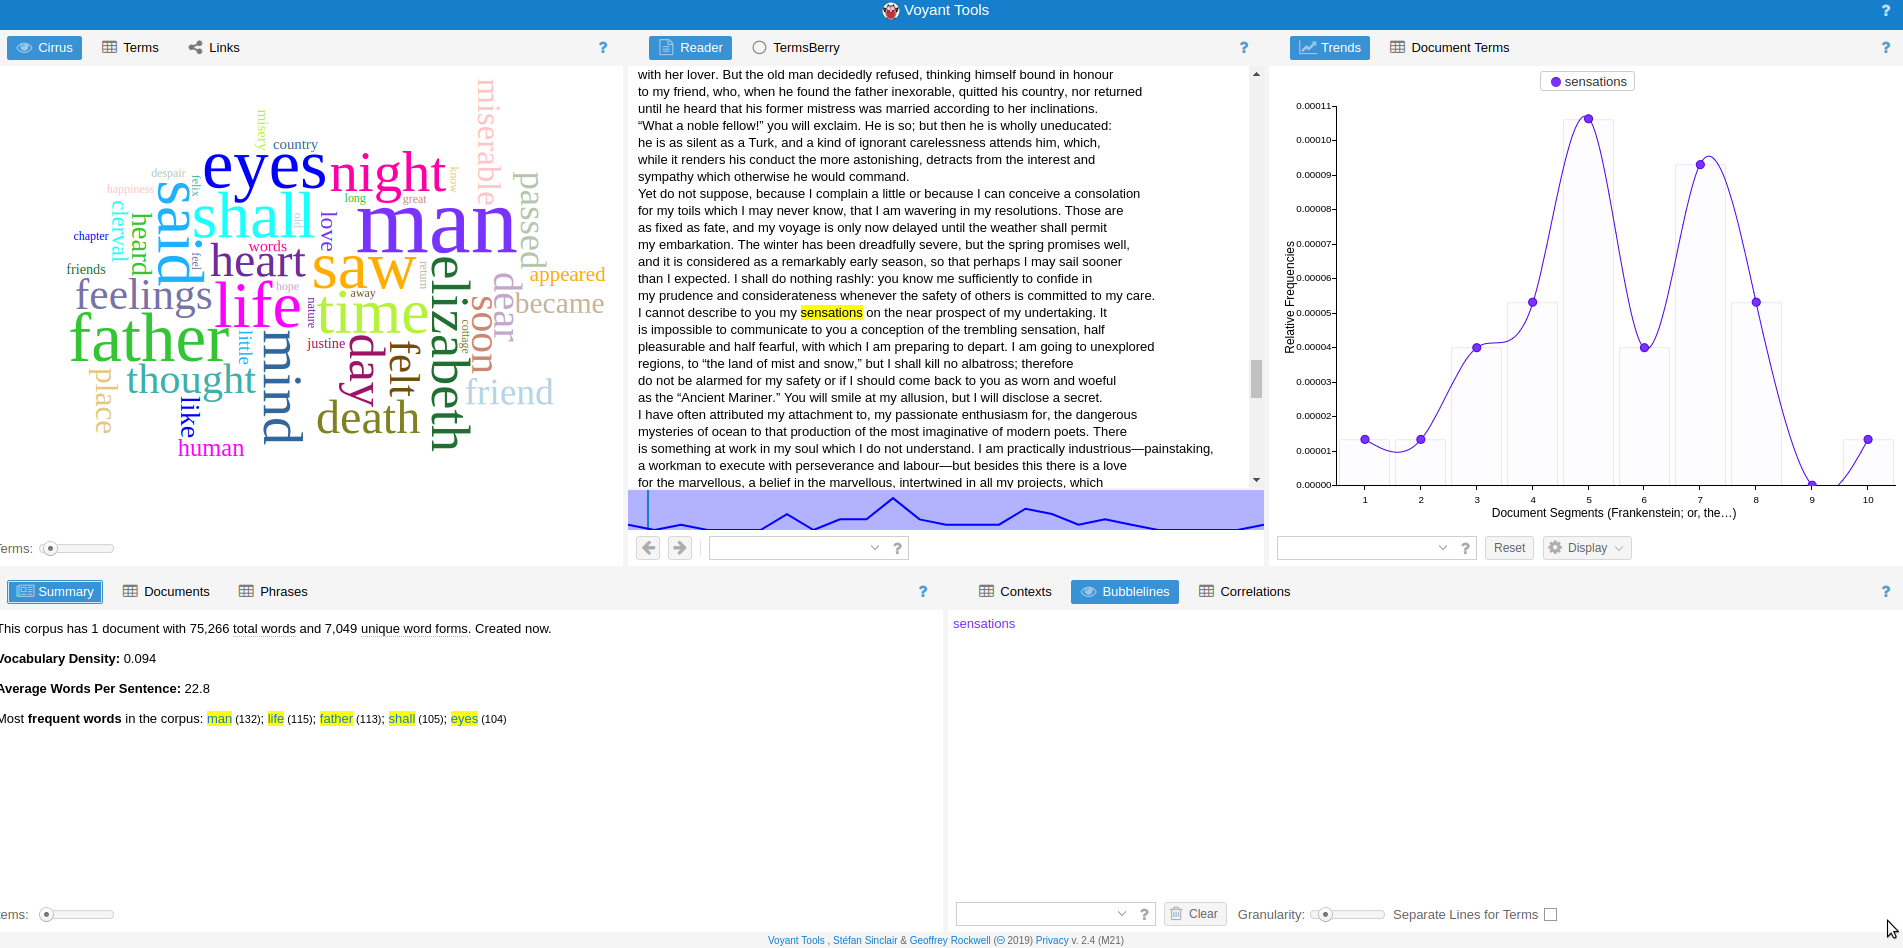
\includegraphics[width=\textwidth]{voyant.png}
% \end{textbox}




% \begin{textbox}{Project Gutenberg Texts}
% \begin{tabular}{r|p{0.8\textwidth}}\scriptsize
%     84 & \href{http://www.gutenberg.org/ebooks/84}{Frankenstein; Or, The Modern Prometheus by Mary Wollstonecraft Shelley} \\
%     6087 & \href{https://www.gutenberg.org/ebooks/6087}{The Vampyre; a Tale by John William Polidori} \\
%     696 & \href{https://www.gutenberg.org/ebooks/696}{The Castle of Otranto by Horace Walpole} \\
%     42 & \href{https://www.gutenberg.org/ebooks/42}{The Strange Case of Dr. Jekyll and Mr. Hyde by Robert Louis Stevenson}
% \end{tabular}

% \end{textbox}





% \begin{textbox}{Key concepts}
% \red{Bag-of-words (BOW)}


% \green{\emph{Zipf's Law}}

% \mycommand{_&§!$§/()$}{code}
% \mycommand{shutdown -h now}{to shutdown}

% \end{textbox}


% %--------------------------------------------------------------
% \section{Programming}

% \subsection{Code boxes}


% % first argument: minted programming language name, for example.. css, c, cpp, etc.
% \begin{codebox}{r}{Code box using R}
% # Install
% install.packages("tm")  # for text mining

% # Load
% library("tm")

% # text <- readLines(file.choose())
% # Read the text file from internet
% filePath <- "http://www.internet.com/text.txt"
% text <- readLines(filePath)

% \end{codebox}


% % first argument: minted programming language name, for example.. css, c, cpp, etc.
% \begin{codebox}{cpp}{Code box using C++}
% for (auto element : vector) 
% {
%     sum += element;
% }
% \end{codebox}

% \newpage
% \section{Smaller Subboxes}
% \subsection{Subboxes}
% %---------------------------------------------
% \begin{multibox}{2} % number of boxes in a row
% \begin{subbox}{subbox}{test}
% \tiny


% \bg{alert}{white}{test} 
% \bggreen{test}\\

% \end{subbox}
% \begin{subbox}{customcolor}{test}
% \scriptsize


% \bgupper{w3schools}{black}{test}\\
% \tiny
% tiny font

% \mycommand{$\lxor$}{XOR}
% \mycommand{$\lor$}{OR}
% \end{subbox}
% \end{multibox}




% %---------------------------------------------
% \begin{multibox}{2} % number of boxes in a row
% \begin{subbox}{subbox}{ Infos}

% \bg{alert}{white}{bla}\\
% \bgupper{w3schools}{black}{XX}\\

% \end{subbox}
% \begin{subbox}{customcolor}{ Infos}

% \end{subbox}
% \end{multibox}


% \begin{textbox}{Subboxes}
% %---------------------------------------------
% \begin{multibox}{2} % number of boxes in a row
% \begin{subbox}{subbox}{test}

% \red{test} 
% \bggreen{test}
% \href{https://latex-ninja.com}{Link}
% \end{subbox}
% \begin{subbox}{customcolor}{test}
% \scriptsize


% \bggreen{test}
% \tiny
% super small font

% \mycommand{$\land$}{AND $\land$}
% \mycommand{$\lor$}{OR $\lor$}
% \end{subbox}
% \end{multibox}

% %---------------------------------------------
% \begin{multibox}{2} % number of boxes in a row
% \begin{subbox}{subbox}{ Info}

% \red{bla}\\
% \bggreen{XX}\\

% \end{subbox}
% \begin{subbox}{customcolor}{Info}

% \end{subbox}
% \end{multibox}
% \end{textbox}


% %--------------------------------------------------------------

% \begin{textbox}{bla}


% \bgupper{w3schools}{black}{test}\\
% \bg{alert}{white}{bla}
% \begin{enumerate}
%     \item \emph{bla}: bla.
%     \item bla.
% \end{enumerate}

% %---------------------------------------------
% \begin{multibox}{3} % number of boxes in a row
% \begin{subbox}{subbox}{test}
% info
% \end{subbox}
% \begin{subbox}{customcolor}{test}
% $p \to q$
% \mycommand{CTRL+C}{copy}
% \end{subbox}
% \begin{subbox}{subbox}{ Infos}
% bla \\
% more text
% \end{subbox}
% \end{multibox}

% %---------------------------------------------
% \begin{multibox}{3} % number of boxes in a row
% \begin{subbox}{subbox}{ Infos}
% info
% \end{subbox}
% \begin{subbox}{customcolor}{ Infos}
% $p \to q$
% \end{subbox}
% \begin{subbox}{subbox}{ Infos}
% bla \\
% more text
% \end{subbox}
% \end{multibox}

% \end{textbox}


% %---------------------------------------------
 \AtNextBibliography{\footnotesize}
 \printbibliography  
 \end{multicols}

\end{document}
